\clearpage

\renewcommand{\thefigure}{\arabic{figure}}
\setcounter{figure}{0}
\renewcommand{\thetable}{\thesection \arabic{table}}
\setcounter{table}{0}
%\renewcommand{\thesection}{A.\arabic{section}}
\setcounter{section}{0}

\appendix
\section{AME Monte Carlo Markov Chain Algorithm}

Given initial values of $\{\bm\beta, \mathbf{a}, \mathbf{b}, \mathbf{U}, \mathbf{V}, \Sigma_{ab}, \rho, \text{ and } \sigma_{\epsilon}^{2}\}$, the algorithm proceeds as follows until convergence:\footnote{Further details on the full conditional distributions and estimation approach underlying AME can be found in \citet{hoff:2021}.}

 \begin{itemize}
  \item sample $\bm\theta \; | \;  \bm\beta, \mathbf{X}, \bm\theta, \mathbf{a}, \mathbf{b}, \mathbf{U}, \mathbf{V}, \Sigma_{ab}, \rho, \text{ and } \sigma_{\epsilon}^{2}$ (Normal)
  \item sample $\bm\beta \; | \;  \mathbf{X}, \bm\theta, \mathbf{a}, \mathbf{b}, \mathbf{U}, \mathbf{V}, \Sigma_{ab}, \rho, \text{ and } \sigma_{\epsilon}^{2}$ (Normal)
  \item sample $\mathbf{a}, \mathbf{b} \; | \; \bm\beta, \mathbf{X}, \bm\theta, \mathbf{U}, \mathbf{V}, \Sigma_{ab}, \rho, \text{ and } \sigma_{\epsilon}^{2}$ (Normal)
  \item sample $\Sigma_{ab} \; | \; \bm\beta, \mathbf{X}, \bm\theta, \mathbf{a}, \mathbf{b}, \mathbf{U}, \mathbf{V}, \rho, \text{ and } \sigma_{\epsilon}^{2}$ (Inverse-Wishart)
  \item update $\rho$ using a Metropolis-Hastings step with proposal $p^{*} | p  \sim$ truncated normal$_{[-1,1]}(\rho, \sigma_{\epsilon}^{2})$
  \item sample $\sigma_{\epsilon}^{2} \; | \; \bm\beta, \mathbf{X}, \bm\theta, \mathbf{a}, \mathbf{b}, \mathbf{U}, \mathbf{V}, \Sigma_{ab}, \text{ and } \rho$ (Inverse-Gamma)
  \item For each $k \in K$:
  \begin{itemize}
    \item Sample $\mathbf{U}_{[,k]} \; | \; \bm\beta, \mathbf{X}, \bm\theta, \mathbf{a}, \mathbf{b}, \mathbf{U}_{[,-k]}, \mathbf{V}, \Sigma_{ab}, \rho, \text{ and } \sigma_{\epsilon}^{2}$ (Normal)
    \item Sample $\mathbf{V}_{[,k]} \; | \; \bm\beta, \mathbf{X}, \bm\theta, \mathbf{a}, \mathbf{b}, \mathbf{U}, \mathbf{V}_{[,-k]}, \Sigma_{ab}, \rho, \text{ and } \sigma_{\epsilon}^{2}$ (Normal)
    \item Sample $\mathbf{D}_{[k,k]}  \; | \; \bm\beta, \mathbf{X}, \bm\theta,\mathbf{a}, \mathbf{b}, \mathbf{U}, \mathbf{V}, \Sigma_{ab}, \rho, \text{ and } \sigma_{\epsilon}^{2}$ (Normal)\footnote{Subsequent to estimation, $\mathbf{D}$ matrix is absorbed into the calculation for $\mathbf{V}$ as we iterate through $K$. }
  \end{itemize}
 \end{itemize}
\newpage

\section{Additional Replication Information}

For each of the replications involving a binary dependent variable we provide a table of coefficient estimates that includes the original GLM estimation and the results from the AME model.  We have adopted for presentation purposes only the use of significance testing on these observational data for facile comparison with the replicated studies.  However, note that we do provide predictive heuristics for these models as well.

% Additionally, for each replication we provide a more detailed visualization illustrating the results of our out-of-sample performance analysis. %For Weeks (2012) we already did so in the main body of the text so we eschew from doing so again here.

\clearpage
\subsection*{Reiter \& Stam (2003)}

Additional information for the Reiter \& Stam (2003) re-estimation.

% latex table generated in R 4.0.3 by xtable 1.8-4 package
% Fri Jul 02 15:14:21 2021
\begin{table}[ht]
\centering
\begingroup\normalsize
\begin{tabular}{lcc}
 Variable & GLM (Logit) & AME \\ 
  \hline
\hline
Intercept & -4.784 & -3.224 \\ 
   & (0.097) & (0.076) \\ 
  Pers/Democ Directed Dyad & 1.026 & 0.252 \\ 
   & (0.14) & (0.066) \\ 
  Democ/Pers Directed Dyad & 0.083 & 0.114 \\ 
   & (0.191) & (0.089) \\ 
  Personal & 0.281 & 0.212 \\ 
   & (0.265) & (0.11) \\ 
  Military & -0.323 & -0.005 \\ 
   & (0.574) & (0.234) \\ 
  Single & -0.677 & -0.033 \\ 
   & (0.144) & (0.081) \\ 
  Democracy & -1.073 & -0.247 \\ 
   & (0.194) & (0.069) \\ 
  Contiguous & 2.912 & 1.311 \\ 
   & (0.09) & (0.038) \\ 
  Major Power & 2.174 & 0.931 \\ 
   & (0.101) & (0.107) \\ 
  Ally & 0.078 & 0.157 \\ 
   & (0.086) & (0.042) \\ 
  Higher/Lower Power Ratio & -0.316 & -0.106 \\ 
   & (0.027) & (0.012) \\ 
  Economically Advanced & -0.175 & 0.057 \\ 
   & (0.131) & (0.055) \\ 
  Years Since Last Dispute & -0.381 & -0.124 \\ 
   & (0.023) & (0.008) \\ 
  Cubic Spline 1 & -0.004 & -0.001 \\ 
   & (0.000) & (0.000) \\ 
  Cubic Spline 2 & 0.002 & 0.001 \\ 
   & (0.000) & (0.000) \\ 
  Cubic Spline 3 & -0.001 & 0.000 \\ 
   & (0.000) & (0.000) \\ 
   \hline
\hline
\end{tabular}
\endgroup
\caption{Parameter comparison for Reiter \& Stam (2003). Standard errors in parentheses.} 
\label{tab:appendix_tableB1_coef}
\end{table}

\FloatBarrier

% \begin{figure}
% 	\centering
% 	\subfigure[AUC]{\label{fig:reiterstamroc}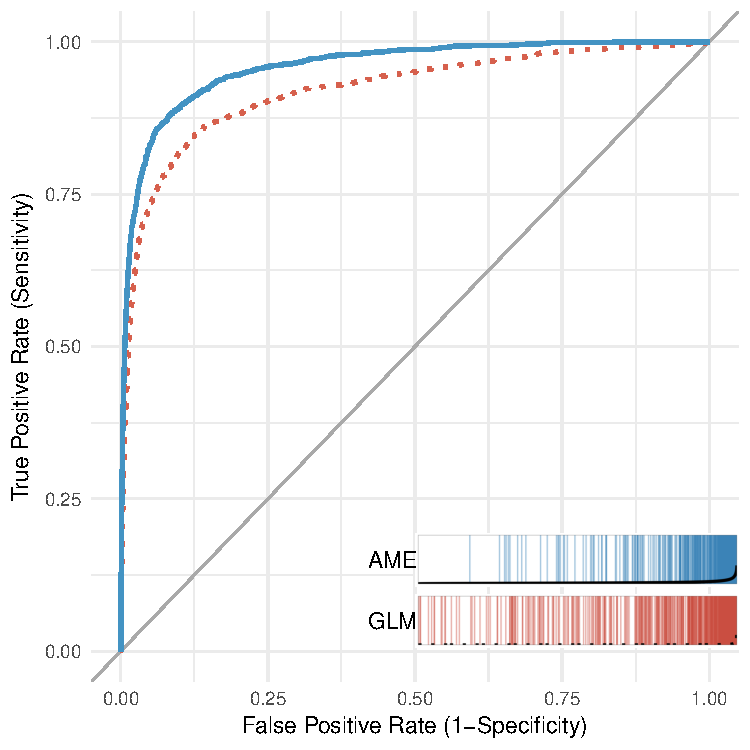
\includegraphics[width=.45\textwidth]{reiter_stam_roc_outSample.pdf}}
% 	\subfigure[Precision and Recall]{\label{fig:reiterstampr}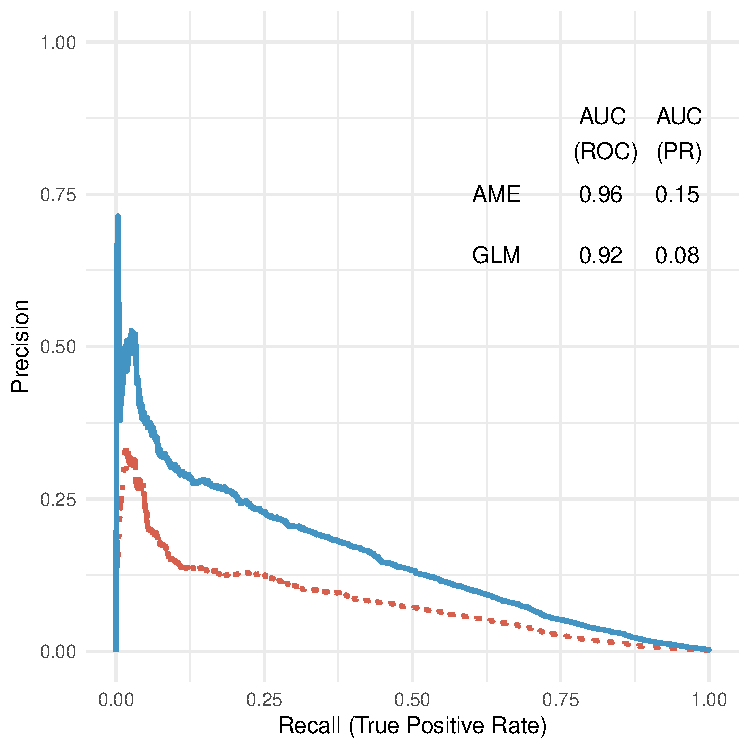
\includegraphics[width=.45\textwidth]{reiter_stam_pr_outSample.pdf}}
% 	\caption{Assessments of out-of-sample predictive performance for Reiter \& Stam (2003) using ROC curves, PR curves, and separation plots.}
% \end{figure}
\FloatBarrier
\clearpage

\subsection*{Weeks (2012)}

Additional information for the Weeks (2012) re-estimation.

% latex table generated in R 4.0.3 by xtable 1.8-4 package
% Fri Jul 02 15:16:41 2021
\begin{table}[ht]
\centering
\begingroup\normalsize
\begin{tabular}{lcc}
 Variable & GLM (Logit) & AME \\ 
  \hline
\hline
(Intercept) & -3.784 & -2.432 \\ 
   & (0.423) & (0.122) \\ 
  Machine & -0.459 & -0.003 \\ 
   & (0.174) & (0.041) \\ 
  Junta & 0.515 & 0.031 \\ 
   & (0.169) & (0.045) \\ 
  Boss & 0.649 & -0.04 \\ 
   & (0.153) & (0.046) \\ 
  Strongman & 0.832 & 0.04 \\ 
   & (0.132) & (0.044) \\ 
  Other Type & 0.147 & -0.001 \\ 
   & (0.132) & (0.034) \\ 
  New/Unstable Regime & -0.312 & -0.042 \\ 
   & (0.092) & (0.033) \\ 
  Democracy Target & 0.185 & 0.025 \\ 
   & (0.115) & (0.026) \\ 
  Military Capabilities Initiator & 5.234 & 0.044 \\ 
   & (1.69) & (0.387) \\ 
  Military Capabilities Target  & 6.34 & -0.938 \\ 
   & (1.675) & (0.477) \\ 
  Low Trade Dependence  & -24.794 & -4.872 \\ 
   & (12.866) & (3.126) \\ 
  Both Major Powers & 1.136 & 1.114 \\ 
   & (0.547) & (0.232) \\ 
  Minor/Major & 0.772 & 0.506 \\ 
   & (0.239) & (0.112) \\ 
  Major/Minor & 0.711 & 0.766 \\ 
   & (0.225) & (0.153) \\ 
  Contiguous & 2.172 & 0.709 \\ 
   & (0.32) & (0.063) \\ 
  Log Dist. Between Capitals & -0.209 & -0.129 \\ 
   & (0.038) & (0.01) \\ 
  Alliance Similarity Dyad  & -0.999 & -0.061 \\ 
   & (0.144) & (0.062) \\ 
  Alliance Similarity With System Leader Initiator & 0.11 & 0.08 \\ 
   & (0.24) & (0.061) \\ 
  Alliance Similarity Leader Target & 0.203 & 0.079 \\ 
   & (0.244) & (0.057) \\ 
  Time Since Last Conflict & -0.229 & -0.067 \\ 
   & (0.018) & (0.006) \\ 
  Spline1 & -0.001 & 0.000 \\ 
   & (0.000) & (0.000) \\ 
  Spline2 & 0.000 & 0.000 \\ 
   & (0.000) & (0.000) \\ 
  Spline3 & 0.000 & 0.000 \\ 
   & (0.000) & (0.000) \\ 
   \hline
\hline
\end{tabular}
\endgroup
\caption{Parameter comparison for Weeks (2012)). Standard errors in parentheses.} 
\label{tab:appendix_tableB2_coef}
\end{table}

\FloatBarrier

% \begin{figure}
% \centering
%   \subfigure[AUC]{\label{fig:weeksauc}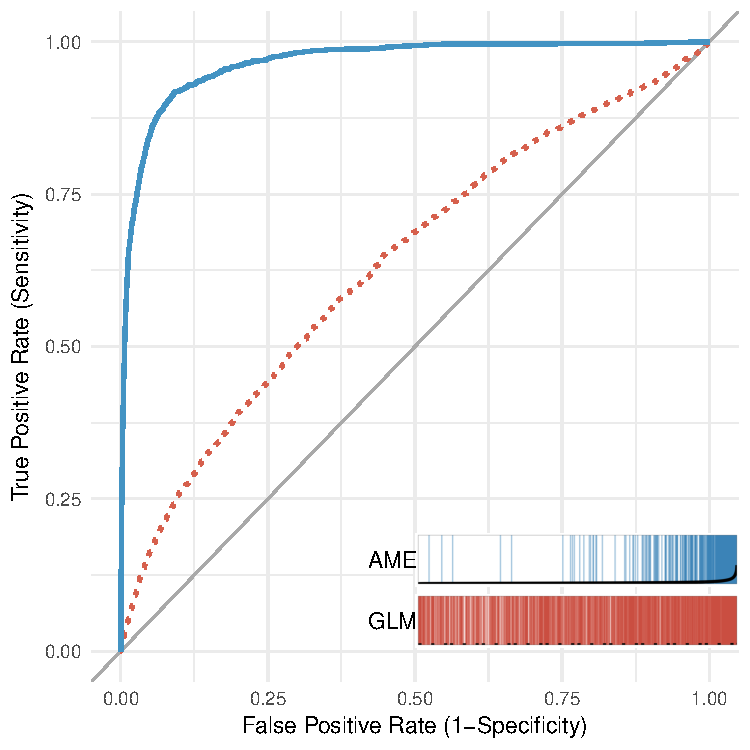
\includegraphics[width=.45\textwidth]{weeks_roc_outSample.pdf}}
%   \subfigure[Precision and Recall]{\label{fig:reitpr}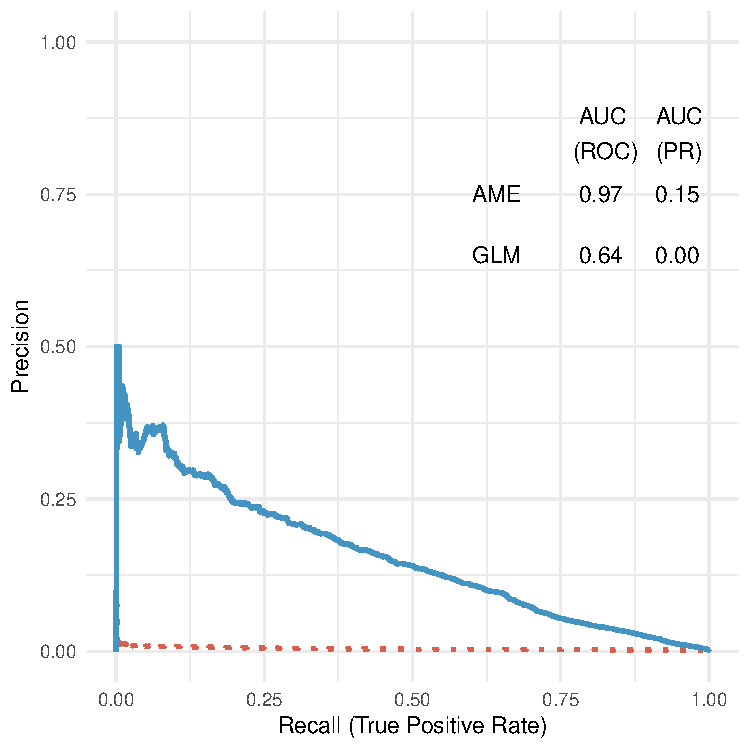
\includegraphics[width=.45\textwidth]{weeks_pr_outSample.pdf}}
%   \caption{Assessments of out-of-sample predictive performance for Weeks (2012) using ROC curves and PR curves}
% \end{figure}
\FloatBarrier
\clearpage

\subsection*{Gibler (2017)}

Additional information for the Gibler (2017) re-estimation.

% latex table generated in R 4.0.3 by xtable 1.8-4 package
% Sat Mar 13 00:09:38 2021
\begin{table}[ht]
\centering
\begingroup\normalsize
\begin{tabular}{lcc}
 Variable & GLM (Logit) & AME \\ 
  \hline
\hline
(Intercept) & -5.826 & -2.755 \\ 
   & (0.366) & (0.038) \\ 
  Allied & 0.133 & 0.076 \\ 
   & (0.102) & (0.023) \\ 
  Joint Democracy & -0.527 & 0.015 \\ 
   & (0.099) & (0.021) \\ 
  Peace Years & -0.261 & -0.061 \\ 
   & (0.016) & (0.004) \\ 
  Spline 1 & -0.001 & 0.000 \\ 
   & (0.000) & (0.000) \\ 
  Spline 2 & 0.000 & 0.000 \\ 
   & (0.000) & (0.000) \\ 
  Spline 3 & 0.000 & 0.000 \\ 
   & (0.000) & (0.000) \\ 
  Contiguity & 2.427 & 0.647 \\ 
   & (0.196) & (0.024) \\ 
  Parity & -0.77 & -0.108 \\ 
   & (0.551) & (0.072) \\ 
  Parity at Entry Year & 2.034 & 0.068 \\ 
   & (0.617) & (0.068) \\ 
  Rivalry & 2.034 & 0.683 \\ 
   & (0.213) & (0.025) \\ 
   \hline
\hline
\end{tabular}
\endgroup
\caption{Parameter comparison for Gibler (2017). Standard errors in parentheses.} 
\label{tab:appendix_tableB3_coef}
\end{table}

\FloatBarrier

% \begin{figure}
% 	\centering
% 	\subfigure[AUC]{\label{fig:giblerroc}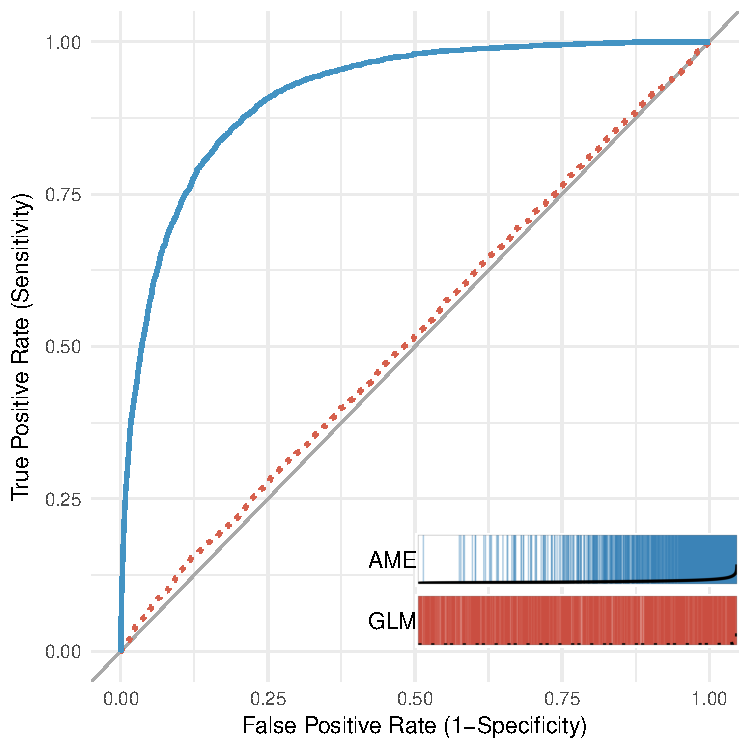
\includegraphics[width=.45\textwidth]{gibler_roc_outSample.pdf}}
% 	\subfigure[Precision and Recall]{\label{fig:giblerpr}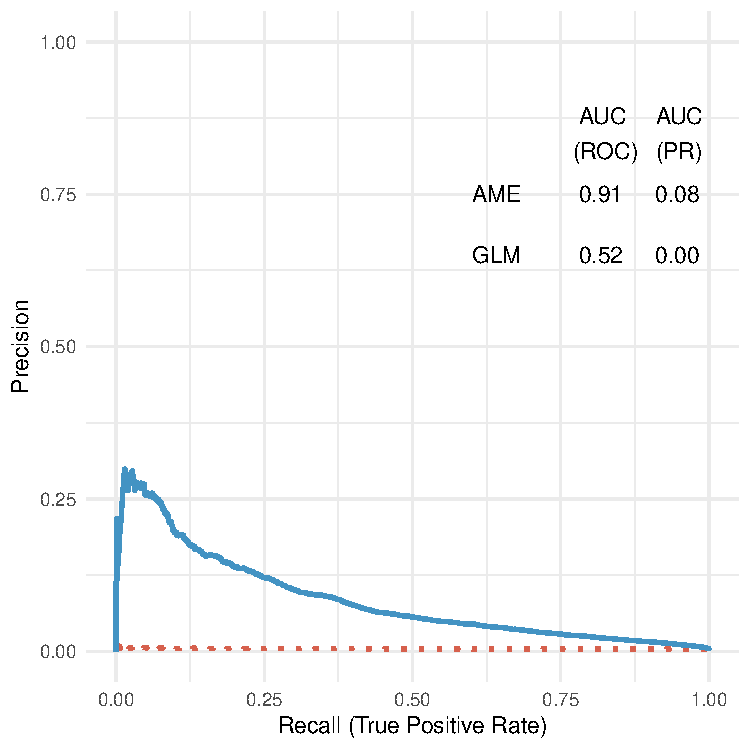
\includegraphics[width=.45\textwidth]{gibler_pr_outSample.pdf}}
% 	\caption{Assessments of out-of-sample predictive performance for Gibler (2017) using ROC curves, PR curves, and separation plots.}
% \end{figure}
\FloatBarrier
\clearpage


\section{Additional Simulations: Non-Linear Data}

Aronow et al note that ``fitting a linear approximation to mildly non-linear data'' can be problematic for dyadic random effect models. We agree on the importance of testing this in the context of the simulation that we posed in the paper. Aronow et al incorporate non-linear misspecification by adding in squared version of the key dyadic homophily variable to the DGP for their simulations: $Y_{i,j} = \beta_{0} + \beta_{1} X_{i,j} + \beta_{2} X_{i,j}^{2} + \epsilon_{i,j}$. Here $X$ is their representation of homophily and is considered observed, while $X^{2}$ is their check for robustness to misspecification and is unobserved. We incorporate the same type of misspecification into our probit simulation setup: $Z_{i,j} =  \mu + \beta X_{i,j} + \gamma W_{i,j} + \epsilon_{i,j}$, where $W$ now instead of being drawn from a separate normal distribution is just the squared version of $X$. For the simulation we set values of $\mu$, $\beta$, and $\gamma$ to -2, 1, and 1, respectively. Results are shown below in Figures~\ref{fig:ameBias_asa} and \ref{fig:ameCalib_asa} below. As in the paper, along the x-axis we implement a standard model that does not take any steps to account for dependencies, AME, and the Oracle model, and as in the paper we find that the AME approach provides a number of benefits in terms of bias and coverage over the standard approach of not dealing with dependencies.

\begin{figure}[ht]
	\centering
	\caption{Regression parameter estimates for the standard, AME, and oracle models from 1,000 simulations. Summary statistics are presented through a traditional box plot, and the estimates from each simulation are visualized as well as points.}
	\label{fig:ameBias_asa}
	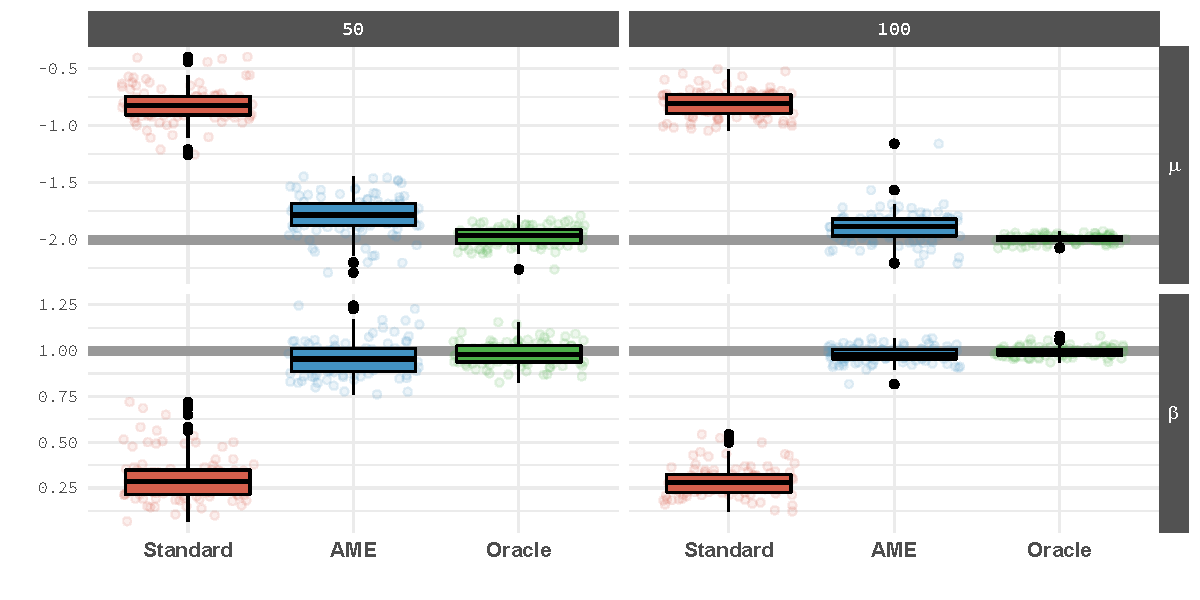
\includegraphics[width=1\textwidth]{graphics/appendix_figureC1.pdf} \\
\end{figure}

\begin{figure}[ht]
	\centering
	\caption{Proportion of times the true value fell within the estimated 95\% confidence interval for the standard, AME, and oracle models from 1,000 simulations.}
	\label{fig:ameCalib_asa}
	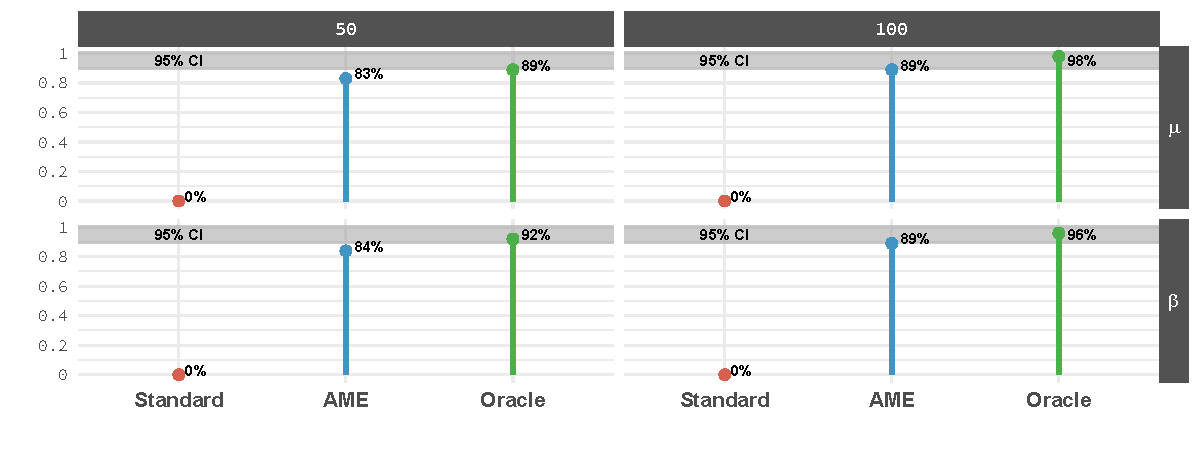
\includegraphics[width=1\textwidth]{graphics/appendix_figureC2.pdf} \\
\end{figure}

\FloatBarrier
\clearpage

\section{Additional Simulations: Correlation with Omitted Variable}

Estimation certainly gets more challenging when the omitted variable is correlated with the observed variable. In the case of normal linear regression, we can show that in general a regression coefficient is unbiased for its ``unconditional effect'', which is the direct effect plus something related to the direct effects of any omitted variables that it is correlated with. For example, suppose in our simulation setup $X_{i,j}$ is correlated with $W_{i,j}$ via the relation $W_{i,j} = \alpha X_{i,j} + e_{i,j}$. Then:

\begin{align*}
  Y_{i,j} & = \mu + \beta X_{i,j} + \gamma W_{i,j} + \epsilon_{i,j} \\
  &= \mu + (\gamma \alpha+\beta ) X_{i,j} + (\gamma Z_{i,j} + \epsilon_{i,j})  \\
  &= \mu + \tilde \beta X_{i,j} + \tilde \epsilon_{i,j}
\end{align*}

The naive model is in some sense still ``correct'' as it is an unbiased estimator of the unconditional (direct plus indirect) effect $\gamma\alpha + \beta$ of $X$ on $Y$. However, there is no way to eliminate this extra bias without making further assumptions about the nature of the omitted variable. Additonally, in the binary case with the probit setup, other sources of bias get introduced as well because of the nonlinearity of the population moments as a function of the parameters. An interesting question is whether or not we can reduce the bias in the network setting by assuming the omitted variable $w_{i,j}$ is the product of latent node-specific factors. An idea related to this is discussed in \citet{minhas:etal:2017:arxiv}.

For now though to show the amount of bias that gets introduced into our setup when $X$ and $W$ are correlated we repeat our simulation exercise but induce varying levels of correlation between $X$ and $W$. Results with $X$ and $W$ correlated at 0.4 and then 0.7 are shown below, respectively.

\begin{figure}[ht]
\caption{Regression parameter estimates for the standard, AME, and oracle models from 1,000 simulations. Summary statistics are presented through a traditional box plot, and the estimates from each simulation are visualized as well as points. $X$ and $W$ are correlated at 0.4 in this case.}
\label{fig:ameBias_corrMed}
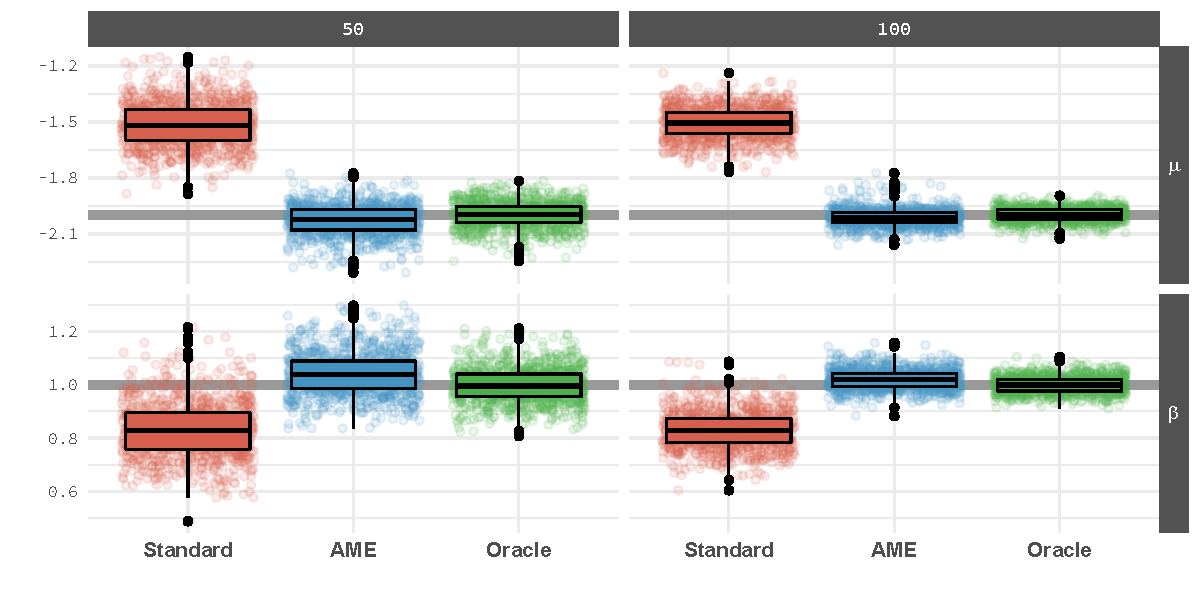
\includegraphics[width=1\textwidth]{graphics/appendix_figureD1a.pdf} \\
\end{figure}

\begin{figure}[ht]
\caption{Regression parameter estimates for the standard, AME, and oracle models from 1,000 simulations. Summary statistics are presented through a traditional box plot, and the estimates from each simulation are visualized as well as points. $X$ and $W$ are correlated at 0.7 in this case.}
\label{fig:ameBias_corrHi}
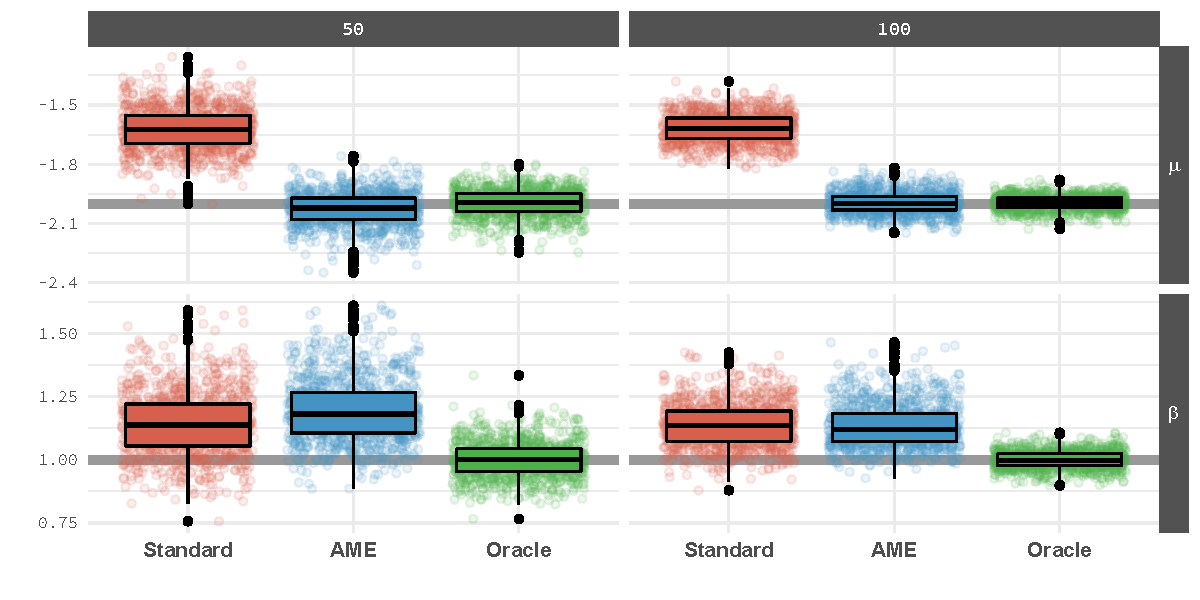
\includegraphics[width=1\textwidth]{graphics/appendix_figureD1b.pdf} \\
\end{figure}

\FloatBarrier
\clearpage

\section{AME Tutorial}

Using the AMEN function requires formatting data into a particular structure. The primary distinction in data formatting is whether the outcome of interest represents a directed or undirected network.

If undirected, the AMEN function has three main inputs:

\begin{itemize}[noitemsep,nolistsep]
    \item Y: a $T$ length \textbf{list} of $n\times n$ adjacency matrices, where $T$ = number of years in the dataset and $n$ = number of nodes in the network.
    \begin{itemize}
      \item An adjacency matrix describes relationships between nodes in a particular year of data. For example, in an adjacency matrix of interstate MIDs, row $i$ and column $j$ takes a value of '1' if country $i$ and country $j$ had a MID in that year, and '0' otherwise. The diagonal in the adjacency matrix is typically missing. Y is a list of these adjacency matrices for the outcome variable, where each element in the list is a different year of data.
    \end{itemize}
    \item Xdyad: a $T$ length \textbf{list} of $n\times n\times p$ arrays, where $p$ = number of dyadic covariates in dataset.
    \begin{itemize}
      \item An array is a data object in R that contains a series of 'stacked' matrices for each year of data. An array of dimension (2, 3, 4), for example, contains 4 rectangular matrices each with 2 rows and 3 columns. Each matrix in the array describes the relationship between nodes with respect to some covariate. For example, for interstate alliances, row $i$ and column $j$ takes a value of '1' if country $i$ and country $j$ had an alliance in that year, and '0' otherwise. An array contains a matrix of this kind for each covariate going into the model. Xdyad is a list of these arrays, where each element in the list is a different year of data.
    \end{itemize}
    \item Xrow: a $T$ length \textbf{list} of $n\times p$ matrices, where $p$ = number of monadic (nodal) covariates in dataset.
    \begin{itemize}
      \item Each matrix in Xrow has the nodes running down the rows and the covariates in the dataset running along the columns. An entry in the matrix captures the value that a node takes on for each covariate in a given year. For example, if column $j$ is GDP per capita and column $k$ is population, then row $i$, column $j$ measures country $i$'s GDP per capita and row $i$, column $k$ measures country $i$'s population in a given year. Xrow is a list of these matrices, where each element in the list is a different year of data.
    \end{itemize}
\end{itemize}

If directed, AMEN further requires:

\begin{itemize}[noitemsep,nolistsep]
    \item Xrow: a $T$ length list of $n\times p$ matrices, where $p$ = number of sender (nodal) covariates in dataset.
    \begin{itemize}
      \item Xrow here is nearly identical to the undirected case. The only difference is that rather than each matrix containing covariate data on all nodes, in the directed context each matrix only contains data on the nodes that are acting as senders in that particular year. Using interstate MIDs as an example, if in 1983 only two countries initiated MIDs, Xrow would only contain data for those two countries (i.e., Xrow would only have two rows).
    \end{itemize}
    \item Xcol: a $T$ length list of $n\times p$ matrices, where $p$ = number of receiver (nodal) covariates in dataset.
    \begin{itemize}
      \item Xcol here is nearly identical to Xrow, except each matrix contains data on receiver nodes, not sender nodes. Using interstate MIDs as an example, if in 1983 only two countries had MIDs initiated against them, Xcol would only contain data for those two countries (i.e., Xcol would only have two rows).
    \end{itemize}
\end{itemize}

Beyond the data inputs, the AMEN function requires additional specification:

\begin{itemize}
    \item model: how to model the outcome variable, e.g., `logit'
    \item symmetric: whether the input network is symmetric
    \item intercept: whether to estimate an intercept
    \item nscan: number of iterations of the Markov chain
    \item burn: burn-in period
    \item odens: thinning interval
    \item R: dimension of the multiplicative effect (referred to as $K$ in the paper)
    \item gof: whether to calculate goodness of fit statistics
\end{itemize}

There is often little theoretical reason to choose a particular value of $\sf{R}$ (above). One strategy is to estimate models at different values of $\sf{R}$ and compare goodness of fit statistics across models. Given the computational time needed for parameter estimates to converge, parallelization strategies are recommended to speed up analysis. In addition, providing AMEN function with starting values, either dictated by theory, previous research, or previous runs can also help speed up convergence time.

The code below presents an example of an AME model running in parallel across 4 different levels of $\sf{R}$. Note also that the model is using starting values from a previous run, defined in \textit{startVals}.

\begin{lstlisting}[language=R]
# running in parallel varying k
imps = 10000 ; brn = 25000 ; ods = 10 ; latDims = 0:3

# Run amen in parallel
library(doParallel) ; library(foreach) ; cl=makeCluster(4) ; registerDoParallel(cl)
foreach(ii=1:length(latDims), .packages=c("amen")) %dopar% {

  # load previous model run
  load(prevModelFiles[ii])
  # extract start vals
  startVals0 = ameFit$'startVals'
  # dump rest
  rm(ameFit)

  ameFit = ame_repL(
    Y=yList,Xdyad=xDyadList,Xrow=NULL,Xcol=NULL,
    model="bin",symmetric=FALSE,intercept=TRUE,R=latDims[ii],
    nscan=imps, seed=1, burn=brn, odens=ods,
    plot=FALSE, print=FALSE, gof=TRUE, startVals=startVals0,
    periodicSave=TRUE )
  save(ameFit, file=paste0('model_k', latDims[ii],'_v2.rda') )
}
stopCluster(cl)
\end{lstlisting}
